\section{Introduction} \label{sec:intro}

The HOMFLY polynomial \cite{HOMFLY, Jones, PT} $P(L)(q, a)$ is an invariant of oriented links in $S^3$, defined by the skein relation
\[
    a^{-1}P(
    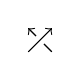
\begin{tikzpicture}[baseline=1]
        \draw[->] (0,0)--(0.3,0.3);
        \draw (0.3,0)--(0.2,0.1);
        \draw[->] (0.1,0.2)--(0,0.3);
    \end{tikzpicture}
    )-a P(
    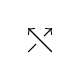
\begin{tikzpicture}[baseline=1]
        \draw[->] (0.3,0)--(0,0.3);
        \draw (0,0)--(0.1,0.1);
        \draw[->] (0.2,0.2)--(0.3,0.3);
    \end{tikzpicture}
    )=(q^{-1}-q)P(
    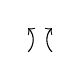
\begin{tikzpicture}[baseline=1]
        \draw [bend right = 45,->] (0,0) to (0,0.3);
        \draw [bend left = 45,->] (0.3,0) to (0.3,0.3);
    \end{tikzpicture}
    ),
\]
and the normalization $P(\text{trivial knot}) = 1$.
The invariant specializes to the Alexander polynomial $\Delta(L)(q) = P(L)(q, 1)$ and to the $sl(N)$ polynomials $P_N(L)(q) = P(L)(q, q^N)$ for $N > 0$. In particular the $sl(2)$ polynomial is the Jones polynomial.

The (reduced) HOMFLY homology $\Hbar^{*,*,*}(L)$ is a categorification of the HOMFLY polynomial, introduced by Khovanov and Rozansky \cite{KR08}.
It is a triply-graded homological link invariant whose graded Euler characteristic is the HOMFLY polynomial $P(L)$.
That is to say, if we denote the Poincar\'e series of $\Hbar(L)$ by
\[
\mathcal{P}(L)(q, a, t) = \sum_{i,j,k} q^ia^jt^{(k-j)/2}\dim \Hbar^{i,\,j,\,k}(L),
\]
then we have $\mathcal{P}(L)(q, a, -1) = P(L)(q,a)$.

The HOMFLY homology is determined for some specific classes of links. For instance, Rasmussen showed that the homology of two-bridge knots are determined by the HOMFLY polynomial and the signature \cite{Ras07}. Mellit and Hogancamp gave recursion formulas to compute the homology of torus links \cite{HM19}.

As for direct computations, although it is technically possible, naive implementation will easily lead to combinatorial explosion. There is a program written by Webster \cite{Web}\footnote{At the time of writing, the program given at the referred URL doesn't seem to work.}, based on the construction using the Rouquier complexes.
%According to Rasmussen \cite{Ras15}, it is capable of computing the homology for knots with braid index $3$.
Rasmussen \cite{Ras15} used this program together with the theoretical machinery he developed, and determined the homologies for all prime knots with up to $9$ crossings. Further computations seem to be out of reach.

In this paper, we give a more effective algorithm to compute the reduced HOMFLY homology of knots, based on Rasmussen's construction \cite{Ras15}. 
By some reinterpretations of the chain complex, we show that the computation is achieved by a sequence of homology computations over $\QQ$. Furthermore, several reduction methods are applicable, which are based on known facts on the HOMFLY homology.

With the implementation of the algorithm \cite{kr-calc} and the braid representations of prime knots provided by \textit{KnotInfo Database} \cite{knotinfo} as the input data, we computed the homology for all prime knots with up to $10$ crossings, and for all prime knots with $11$ crossings and braid length up to $13$ (the bolded parts in \Cref{table:targets}).

\begin{table}[t]
\centering
\begin{tabular}{r|rrrrrrr}
$n \setminus l$	& $\leq 11$	& $12$ & $13$ & $14$ & $15$ & $16$ & $17$\\
\hline
$\leq 8$ & $\mathbf{35}$ \\
$9$ & $\mathbf{43}$ & $\mathbf{5}$ & & $\textbf{1}$ \\
$10$ & $\mathbf{126}$ & $\mathbf{31}$ & $\textbf{2}$ & $\textbf{6}$ \\
$11$ & $\mathbf{237}$ & $\mathbf{135}$ & $\textbf{74}$ & $81$ & $14$ & $9$ & $2$\\
\end{tabular}
\caption{Targets of computation\\ ($n$: crossing number, $l$: braid length)}
\label{table:targets}
\vspace{1em}
\end{table}

\begin{table}[t]
\begin{minipage}{.5\linewidth}
\centering
\begin{tabular}{l|ll}
$k \setminus j$	& $4$	& $6$ \\
\hline
$4$	& $q^{-4}$	&  \\
$0$	& $1$	& $q^{-2}$ \\
$-4$	& $q^4$	& $q^2$ \\
\end{tabular}
\vspace{2.5em}
\end{minipage}%
\begin{minipage}{.5\linewidth}
\centering
\begin{tabular}{l|lll}
$k \setminus j$	& $2$    & $4$	& $6$ \\
\hline
$2$ & $q^{-2}$ &  &  \\
$0$ & $q^{-2}$ & $q^{-4}$ &  \\
$-2$ & $q^{2}$ & $1$ &  \\
$-4$ & $q^{2}$ & $2$ & $q^{-2}$ \\
$-8$ &  & $q^{4}$ & $q^{2}$ \\
\end{tabular}
\end{minipage} 
\caption{$H(5_1)$ and $H(m(10_{132}))$}
\label{table:compare}
\end{table}




Observations on the results give direct proofs of some known facts. \Cref{table:compare} shows the reduced HOMFLY homology of $5_1$ and $m(10_{132})$\footnote{$\Hbar(10_{132})$ is computed in \cite{DGR} with the assumption that their conjecture is true.}, where $m(\cdot)$ indicates mirroring of knots. It is known that $P(5_1) = P(m(10_{132}))$ but we obviously see that $\Hbar(5_1) \neq \Hbar(m(10_{132}))$. This implies that the reduced HOMFLY homology is strictly stronger than the HOMFLY polynomial (as verified in several contexts, for example, see \cite{Kawamuro}). This pair appears in \cite{BarNatan:2002} as an example that the two knots has the same Jones polynomial but distinct Khovanov homology. $11n_{79}$ and $m(11n_{138})$ gives another such pair. 

Another observation is that the Conway knot $11n_{34}$ and the Kinoshita--Terasaka knot $11n_{42}$ have identical reduced HOMFLY homology. This is proved in \cite{MV08} using spectral sequence arguments. The result is interesting in that the two knots have distinct knot Floer homology \cite{OS04}, while it is conjectured that there is a spectral sequence from the reduced HOMFLY homology to the knot Floer homology \cite{DGR}. More observations are given in \Cref{sec:comptuations}. The whole computation results 
can be found at \cite{kr-calc}.

Our original motivation for developing an effective computer program was to investigate how the homology $\Hbar(D)$ defined in \cite{Ras15} varies among diagrams $D$ of the same link $L$. 
Although $\Hbar(D)$ is defined for an arbitrary link diagrams, its invariance is only proved for braidlike Reidemeister moves, and hence the reduced HOMFLY homology $\Hbar(L)$ is defined as $\Hbar(D)$ for a \textit{braid closure diagram} $D$ of $L$. 
In fact, it is known that $\Hbar(D)$ is generally \textit{not} invariant under the RIIb move (\Cref{fig:RIIb}) \cite{Abel17, Nak20}.

\afterpage{
\begin{figure}[t]
    \centering
    

\tikzset{every picture/.style={line width=0.75pt}} %set default line width to 0.75pt        

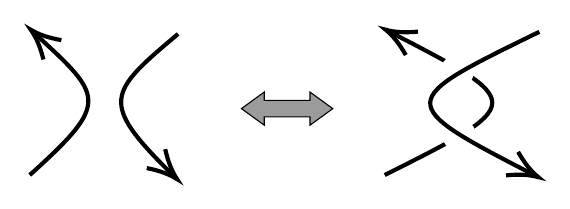
\begin{tikzpicture}[x=0.75pt,y=0.75pt,yscale=-1,xscale=1]
%uncomment if require: \path (0,109); %set diagram left start at 0, and has height of 109

%Curve Lines [id:da9625826323139346] 
\draw [color={rgb, 255:red, 0; green, 0; blue, 0 }  ,draw opacity=1 ][line width=1.5]    (27,88) .. controls (66.2,52.72) and (62.18,50.09) .. (29.53,19.88) ;
\draw [shift={(27.5,18)}, rotate = 402.85] [color={rgb, 255:red, 0; green, 0; blue, 0 }  ,draw opacity=1 ][line width=1.5]    (14.21,-6.37) .. controls (9.04,-2.99) and (4.3,-0.87) .. (0,0) .. controls (4.3,0.87) and (9.04,2.99) .. (14.21,6.37)   ;
%Curve Lines [id:da8544856752658218] 
\draw [color={rgb, 255:red, 0; green, 0; blue, 0 }  ,draw opacity=1 ][line width=1.5]    (95.77,87.82) .. controls (60.17,52.83) and (64.69,48.42) .. (98.5,20) ;
\draw [shift={(98,90)}, rotate = 224.24] [color={rgb, 255:red, 0; green, 0; blue, 0 }  ,draw opacity=1 ][line width=1.5]    (14.21,-6.37) .. controls (9.04,-2.99) and (4.3,-0.87) .. (0,0) .. controls (4.3,0.87) and (9.04,2.99) .. (14.21,6.37)   ;
%Left Right Arrow [id:dp02644365779692881] 
\draw  [fill={rgb, 255:red, 155; green, 155; blue, 155 }  ,fill opacity=1 ] (129,56) -- (140,48) -- (140,52) -- (162,52) -- (162,48) -- (173,56) -- (162,64) -- (162,60) -- (140,60) -- (140,64) -- cycle ;
%Curve Lines [id:da8815340708073711] 
\draw [color={rgb, 255:red, 0; green, 0; blue, 0 }  ,draw opacity=1 ][line width=1.5]    (198,88) .. controls (267.3,53.35) and (266.03,53) .. (200.51,19.04) ;
\draw [shift={(198.5,18)}, rotate = 387.40999999999997] [color={rgb, 255:red, 0; green, 0; blue, 0 }  ,draw opacity=1 ][line width=1.5]    (14.21,-6.37) .. controls (9.04,-2.99) and (4.3,-0.87) .. (0,0) .. controls (4.3,0.87) and (9.04,2.99) .. (14.21,6.37)   ;
%Shape: Circle [id:dp7918407891980368] 
\draw  [draw opacity=0][fill={rgb, 255:red, 255; green, 255; blue, 255 }  ,fill opacity=1 ] (225,38) .. controls (225,33.58) and (228.58,30) .. (233,30) .. controls (237.42,30) and (241,33.58) .. (241,38) .. controls (241,42.42) and (237.42,46) .. (233,46) .. controls (228.58,46) and (225,42.42) .. (225,38) -- cycle ;
%Shape: Circle [id:dp48274841693443793] 
\draw  [draw opacity=0][fill={rgb, 255:red, 255; green, 255; blue, 255 }  ,fill opacity=1 ] (226,69) .. controls (226,64.58) and (229.58,61) .. (234,61) .. controls (238.42,61) and (242,64.58) .. (242,69) .. controls (242,73.42) and (238.42,77) .. (234,77) .. controls (229.58,77) and (226,73.42) .. (226,69) -- cycle ;
%Curve Lines [id:da344766333551638] 
\draw [color={rgb, 255:red, 0; green, 0; blue, 0 }  ,draw opacity=1 ][line width=1.5]    (268.9,87.4) .. controls (202.05,52.99) and (204.04,52.49) .. (272.5,19) ;
\draw [shift={(272,89)}, rotate = 207.22] [color={rgb, 255:red, 0; green, 0; blue, 0 }  ,draw opacity=1 ][line width=1.5]    (14.21,-6.37) .. controls (9.04,-2.99) and (4.3,-0.87) .. (0,0) .. controls (4.3,0.87) and (9.04,2.99) .. (14.21,6.37)   ;




\end{tikzpicture}
    \caption{RIIb move}\label{fig:RIIb}
\end{figure}
}

Compared with the fact that the HOMFLY polynomial $P(L)$ \textit{can} be computed from arbitrary link diagrams, a natural question arises:

\begin{question} \label{question:refine-H}
    Is it possible to refine the construction of the HOMFLY homology so that it can be computed directly from arbitrary link diagrams?
\end{question}

Currently we haven't obtained an answer to this question. We expect that observations on computational results will help us find a clue. More considerations on general link diagrams are given in the final section.

This paper is organized as follows. In \Cref{sec:prelim}, we review the definition of the reduced HOMFLY homology $\Hbar(L)$ given by Rasmussen in \cite{Ras15}. We also recall several important properties of $\Hbar(L)$ which are essential in proving the finiteness of the algorithm. In \Cref{sec:algo} we describe the proposed algorithm, and in \Cref{sec:comptuations} we discuss the computational results. Finally in \Cref{sec:future} we discuss future prospects, regarding the conjecture of \cite{DGR} and the homology $\Hbar(D)$ for general link diagrams. 